\documentclass{article}

\usepackage{graphicx}
\usepackage{tikz}
\usepackage{tikzsymbols}
\usetikzlibrary{calc,patterns,shapes.geometric}
\pagestyle{empty}
\usepackage[margin=0pt]{geometry}
\geometry{papersize={14in,12in}}

\def\centerarc[#1](#2)(#3:#4:#5){\draw[#1] ($(#2)+({#5*cos(#3)},{#5*sin(#3)})$) arc (#3:#4:#5);}

\begin{document}
	\begin{figure}
		\centering
		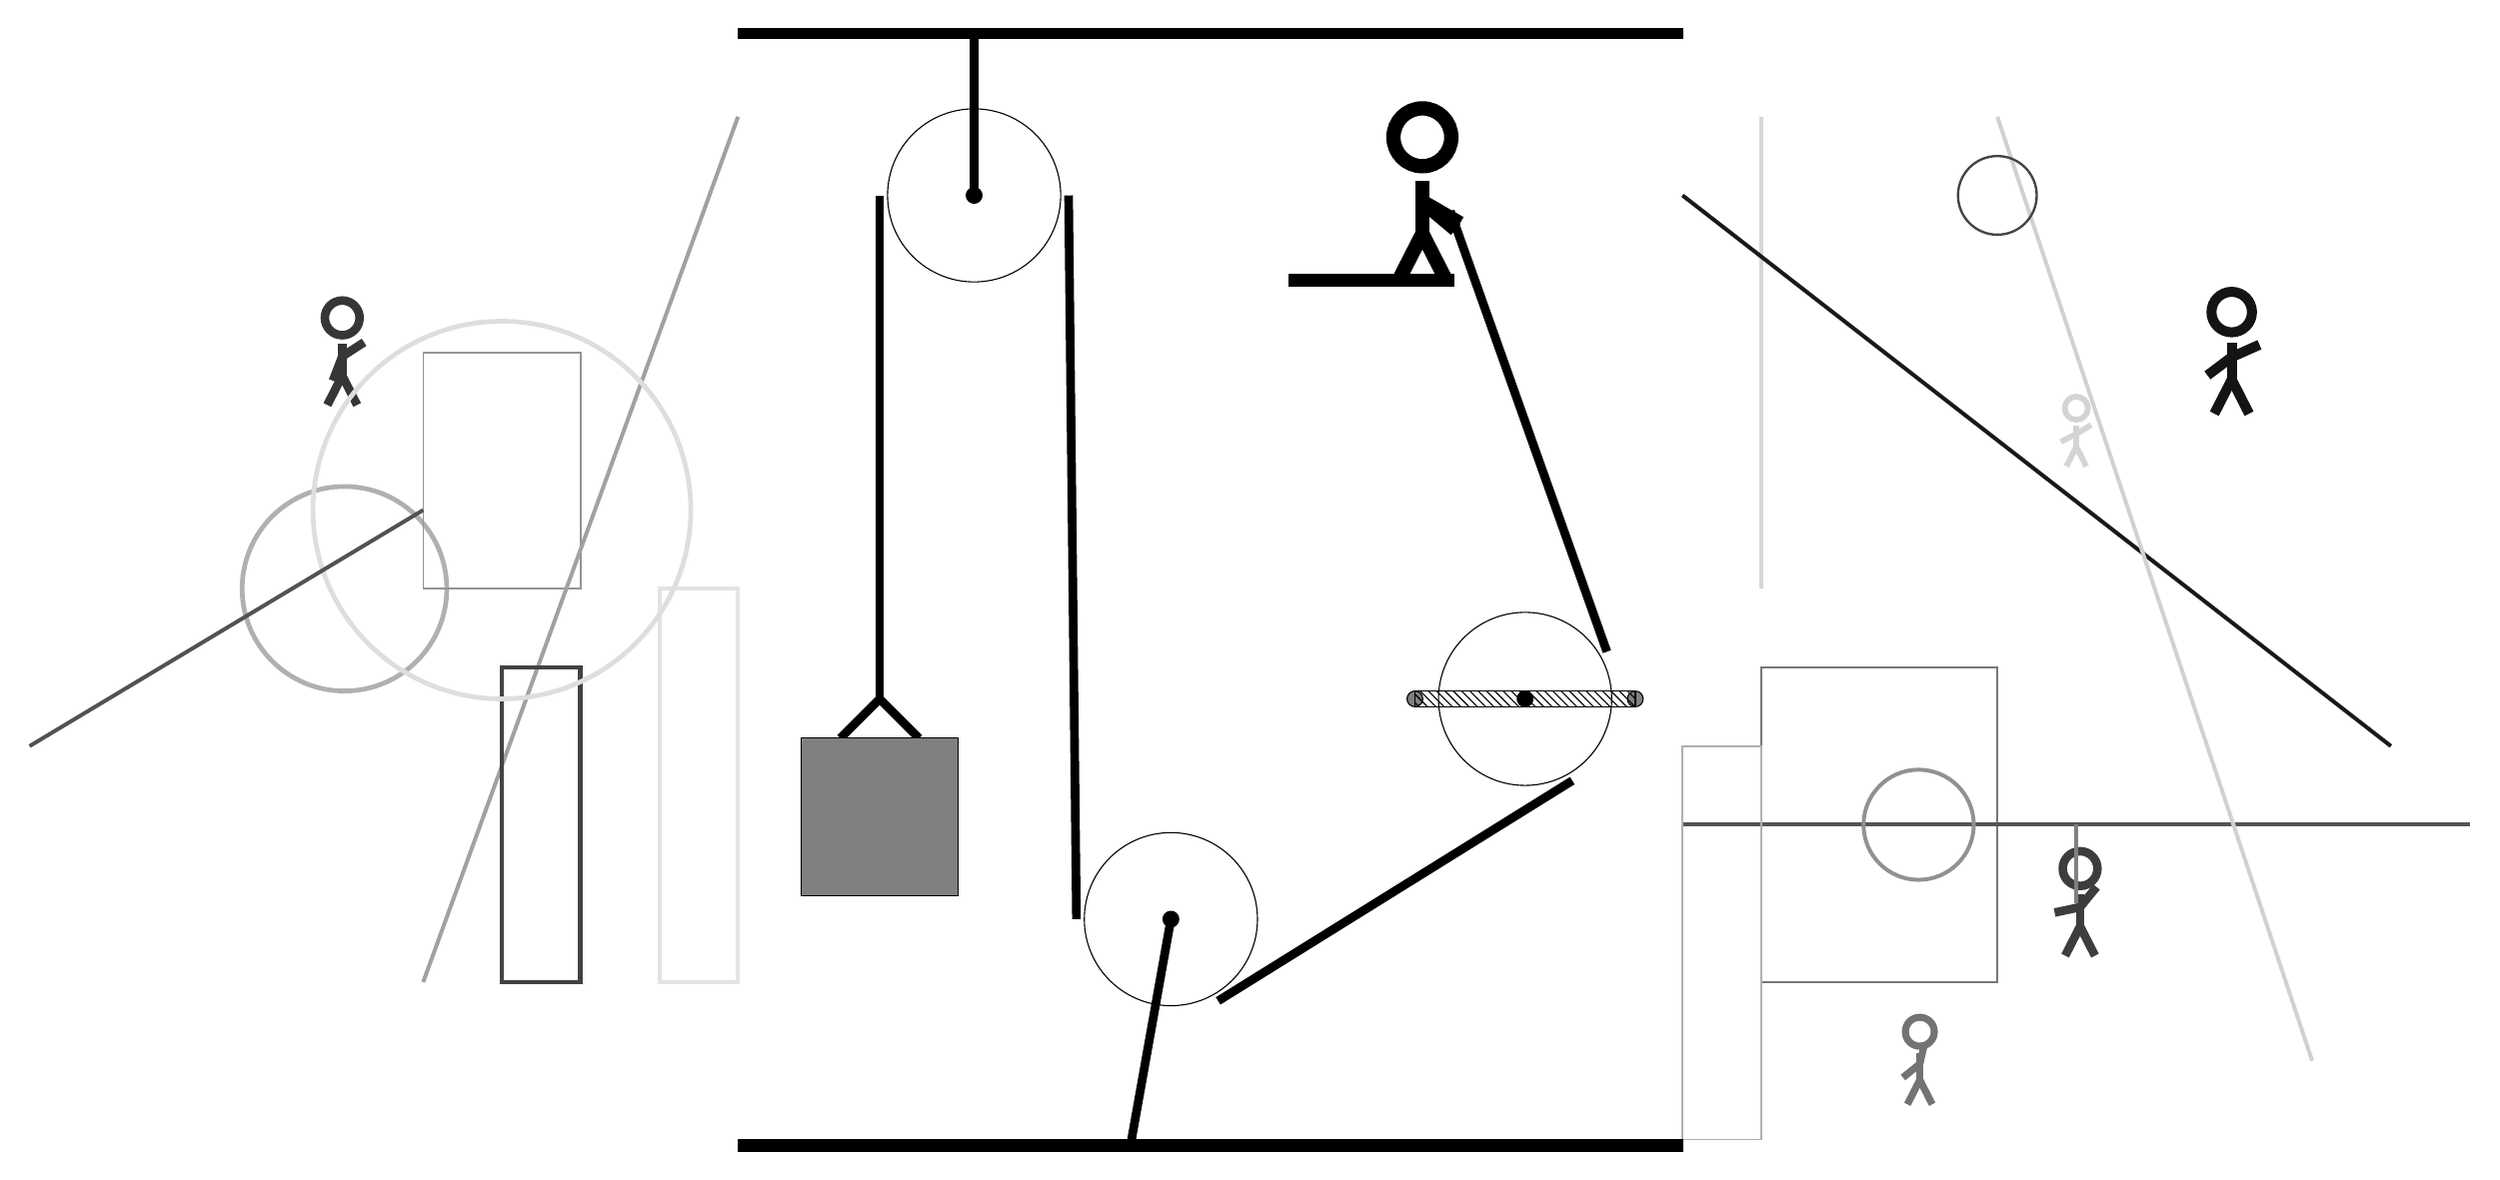
\begin{tikzpicture}
			%%%%% START %%%%%
			
			\draw[fill=black] (-2, 14) rectangle (10, 14.125);
			
			\draw (1, 12) circle (1.1);
			\draw[fill=black] (1, 12) circle (0.1);
			\draw[line width=1.1mm] (1, 14) -- (1, 12);
			
			\draw (3.5, 2.8) circle (1.1);
			\draw[fill=black] (3.5, 2.8) circle (0.1);
			\draw[line width=1.1mm] (3.5, 2.8) -- (3.0, 0);
			
			\draw[fill=white](8, 5.6) circle (1.1);
			\draw[fill=black] (8, 5.6) circle (0.1);
			\draw[fill=black!50] (9.4, 5.6) circle (0.1);
			\draw[fill=black!50] (6.6, 5.6) circle (0.1);
			\draw[pattern=north west lines, pattern color=black] (6.6, 5.7) rectangle (9.4, 5.5);
			
			\draw [line width=0.6mm, color=black!31](-7, 7) circle (1.3);
			
			\draw[line width=0.5mm, color=black!16](11, 7) -- (11, 13);
			\draw[line width=0.3mm, color=black!53] (11, 2) rectangle (14, 6);
			\node[line width=0.5mm, color=black!76] at (15, 3) {\Strichmaxerl[6][12][51]};
			\node[line width=0.3mm, color=black!55] at (13, 1) {\Strichmaxerl[5][39][77]};
			\node[line width=0.6mm, color=black!79] at (-7, 10) {\Strichmaxerl[6][69][33]};
			\draw[line width=0.2mm, color=black!42] (-4, 7) rectangle (-6, 10);
			\draw[line width=0.5mm, color=black!67](10, 4) -- (20, 4);
			\draw[line width=0.5mm, color=black!37](-6, 2) -- (-2, 13);
			
			\draw[line width=0.5mm, color=black!90](10, 12) -- (19, 5);
			\draw[line width=0.5mm, color=black!50](15, 3) -- (15, 4);
			\draw [line width=0.3mm, color=black!75](19, 4) circle (0.0);
			\draw[line width=0.5mm, color=black!11] (-3, 2) rectangle (-2, 7);
			\node[line width=0.2mm, color=black!17] at (15, 9) {\Strichmaxerl[4][27][31]};
			\draw [line width=0.5mm, color=black!43](13, 4) circle (0.7);
			\draw[line width=0.5mm, color=black!18](14, 13) -- (18, 1);
			
			\draw[line width=0.2mm, color=black!31] (10, 5) rectangle (11, 0);
			
			\draw [line width=0.3mm, color=black!73](14, 12) circle (0.5);
			\node[line width=0.2mm, color=black!92] at (17, 10) {\Strichmaxerl[7][37][24]};
			
			\draw[line width=0.6mm, color=black!74] (-4, 2) rectangle (-5, 6);
			\draw [line width=0.6mm, color=black!13](-5, 8) circle (2.4);
			\draw[line width=0.5mm, color=black!68](-6, 8) -- (-11, 5);
			
			
			\draw[line width=1.1mm](-0.7, 5.1) --  (-0.2, 5.6) -- (0.3, 5.1);
			\draw[fill=black!50] (-1.2, 5.1) rectangle (0.8, 3.1);
			
			\draw[line width=1.1mm](-0.2, 12) -- (-0.2, 5.6);
			\centerarc[line width=1.1mm](1, 12)(180:0:1.2000000000000002)
			\draw[line width=1.1mm](2.2, 12) -- (2.3, 2.8);
			\centerarc[line width=1.1mm](3.5, 2.8)(180:300:1.2000000000000002);
			\draw[line width=1.1mm](4.1, 1.7608) -- (8.6, 4.5608);
			\centerarc[line width=1.1mm](8, 5.6)(300:390:1.2000000000000002);
			\draw[line width=1.1mm](9.0392, 6.2) -- (7.05, 11.8);
			
			\node at (6.75, 12) {\Strichmaxerl[10][-220][-30]};
			\draw[fill=black] (5, 11) rectangle (7.1, 10.85);
			
			\draw[fill=black] (-2, 0) rectangle (10, -0.15);
			
			%%%%% END %%%%%
		\end{tikzpicture}
	\end{figure}	
\end{document}